

\documentclass[12pt]{article}
\usepackage{amsmath}
\usepackage{latexsym}
\usepackage{amsfonts}
\usepackage[normalem]{ulem}
\usepackage{array}
\usepackage{amssymb}
\usepackage{graphicx}
\usepackage[backend=biber,
style=numeric,
sorting=none,
isbn=false,
doi=false,
url=false,
]{biblatex}\addbibresource{bibliography.bib}

\usepackage{subfig}
\usepackage{wrapfig}
\usepackage{wasysym}
\usepackage{enumitem}
\usepackage{adjustbox}
\usepackage{ragged2e}
\usepackage[svgnames,table]{xcolor}
\usepackage{tikz}
\usepackage{longtable}
\usepackage{changepage}
\usepackage{setspace}
\usepackage{hhline}
\usepackage{multicol}
\usepackage{tabto}
\usepackage{float}
\usepackage{multirow}
\usepackage{makecell}
\usepackage{fancyhdr}
\usepackage[toc,page]{appendix}
\usepackage[hidelinks]{hyperref}
\usetikzlibrary{shapes.symbols,shapes.geometric,shadows,arrows.meta}
\tikzset{>={Latex[width=1.5mm,length=2mm]}}
\usepackage{flowchart}\usepackage[paperheight=11.0in,paperwidth=8.5in,left=0.59in,right=0.62in,top=0.39in,bottom=0.98in,headheight=1in]{geometry}
\usepackage[utf8]{inputenc}
\usepackage[T1]{fontenc}
\TabPositions{0.49in,0.98in,1.47in,1.96in,2.45in,2.94in,3.43in,3.92in,4.41in,4.9in,5.39in,5.88in,6.37in,6.86in,}

\urlstyle{same}




% 1) Section
% 1.1) SubSection
% 1.1.1) SubSubSection
% 1.1.1.1) Paragraph
% 1.1.1.1.1) Subparagraph


\setcounter{tocdepth}{5}
\setcounter{secnumdepth}{5}





\setlistdepth{9}
\renewlist{enumerate}{enumerate}{9}
		\setlist[enumerate,1]{label=\arabic*)}
		\setlist[enumerate,2]{label=\alph*)}
		\setlist[enumerate,3]{label=(\roman*)}
		\setlist[enumerate,4]{label=(\arabic*)}
		\setlist[enumerate,5]{label=(\Alph*)}
		\setlist[enumerate,6]{label=(\Roman*)}
		\setlist[enumerate,7]{label=\arabic*}
		\setlist[enumerate,8]{label=\alph*}
		\setlist[enumerate,9]{label=\roman*}

\renewlist{itemize}{itemize}{9}
		\setlist[itemize]{label=$\cdot$}
		\setlist[itemize,1]{label=\textbullet}
		\setlist[itemize,2]{label=$\circ$}
		\setlist[itemize,3]{label=$\ast$}
		\setlist[itemize,4]{label=$\dagger$}
		\setlist[itemize,5]{label=$\triangleright$}
		\setlist[itemize,6]{label=$\bigstar$}
		\setlist[itemize,7]{label=$\blacklozenge$}
		\setlist[itemize,8]{label=$\prime$}

\setlength{\topsep}{0pt}\setlength{\parskip}{8.04pt}
\setlength{\parindent}{0pt}




\renewcommand{\arraystretch}{1.3}






\begin{document}
\begin{Center}
{\fontsize{14pt}{16.8pt}\selectfont \textbf{ESTACIONAMIENTO AUTOMATIZADO }\par}
\end{Center}\par

\begin{Center}
\textbf{SISTEMAS ELECTRONICOS DE INTERFAZ}
\end{Center}\par

\begin{Center}
\textbf{\textit{PRIMER AVANCE DE PROYECTO}}
\end{Center}\par


\vspace{\baselineskip}



\begin{figure}[H]
	\begin{Center}
		
\includegraphics[width=5.24in,height=6.06in]{./media/image1.png}
	\end{Center}
\end{figure}



\par

\begin{Center}
{\fontsize{10pt}{12.0pt}\selectfont \textbf{INTEGRANTES}\par}
\end{Center}\par

\begin{Center}
{\fontsize{10pt}{12.0pt}\selectfont BARRERA VÁZQUEZ OMAR\par}
\end{Center}\par

\begin{Center}
{\fontsize{10pt}{12.0pt}\selectfont ESPARZA CABRERA DAVID\par}
\end{Center}\par

\begin{Center}
{\fontsize{10pt}{12.0pt}\selectfont MÁRQUEZ MÁRQUEZ AMAIRANI IVETTE\par}
\end{Center}\par

\begin{Center}
{\fontsize{10pt}{12.0pt}\selectfont MUÑOZ JUÁREZ ALAN ANTONIO\par}
\end{Center}\par

\begin{Center}
{\fontsize{10pt}{12.0pt}\selectfont RUIZ TINOCO GIOVANNI DANIEL\par}
\end{Center}\par


\vspace{\baselineskip}
\textbf{Planteamiento del problema }\par

En la actualidad la necesidad de transportarse es cada vez mayor y a causa de la economía el principal medio de transporte en zonas de alto índice de robo son las motocicletas, estas son adquiridas un precio accesible e incluso a crédito pero dado que estas características no cuentan con un buen sistema antirrobo (como lo son alarmas) por lo que eso las vuelve el principal objetivo de los llamados $``$amantes de lo ajeno$"$  de ahí surge nuestro proyecto el cual tiene como finalidad mantener estos medios de transporte más protegidos ante posibles intentos de robo dado que la mayoría de usuarios de estos medios de transporte no suelen contar con la capacidad adquisitiva suficiente para simplemente volver a comprar otro vehículo, para eso con la ayuda de una plataforma inteligente que atraviese puntos clave de la motocicleta evitando de esta forma el ser removida, además de contar con sistemas de identificación inteligentes para evitar posibles intentos de suplantación del nuestros usuarios. Los altos índices delincuencia y la falta de sistemas efectivos antirrobo genera este tipo de situaciones por ello partimos del supuesto de tener vehículos que no cuentan con un sistema confiable de protección.\par

\textbf{Formulación del problema}\par

Este robo está en aumento dado que la venta de motocicletas en la zona en la que nos enfocaremos está en aumento y por ello se vuelve aún más vulnerable este tipo de vehículo por ser un foco de interés. ¿Cuáles de los sistemas de la motocicleta que la vuelven vulnerable?, ¿Qué situaciones son las más propicias para el robo del vehículo?, ¿Costo del servicio?, ¿Vulnerabilidad por Posibles Factores externos?\par

\textbf{Objetivo general }\par

Diseñar un estacionamiento inteligente el cual brinde la seguridad que necesitan nuestros clientes al aparcar sus motocicletas, aplicando así el concepto de automatización. \par

\textbf{Objetivos del proyecto}\par

\begin{itemize}
	\item Diseñar una interfaz a través de una tarjeta programable la cual nos permita almacenar los datos de nuestros clientes utilizando un servidor como base datos. \par

	\item Producir un prototipo a escala para corroborar que nuestra interfaz funciona correctamente. \par

	\item Elaborar finalmente el prototipo a tamaño real para exponerlo ante el comité. 
\end{itemize}\par

\textbf{Justificación}\par

Los motivos que nos llevaron a realizar\ este proyecto se centran en que existen sectores vulnerables al robo de motocicletas en la zona de metropolitana de Guadalajara, por ello se recurre a tomar la iniciativa de crear un sistema automatizado.  \par

\textbf{Delimitación}\par

La delimitación en el proyecto "estacionamientos inteligentes" la focalización de los estacionamientos inteligentes está centrado para un área urbana como lo es la zona metropolitana, que cuenta con casi 4000 estacionamientos privados de centros comerciales e instituciones públicas y privadas, los cuales carecen de aparcamiento. La idea es llegar a la mayor cantidad posible de estacionamientos en el área metropolitana de Guadalajara y como un mínimo al área perteneciente al municipio de Tlajomulco de Zúñiga y sus comunidades colaterales.\par


\vspace{\baselineskip}

\vspace{\baselineskip}

\vspace{\baselineskip}

\vspace{\baselineskip}
\textbf{Matriz de posibles materiales y costos}\par






\begin{table}[H]
 			\centering
\begin{tabular}{p{3.0in}p{3.0in}}
\hline
%row no:1
\multicolumn{2}{|p{6.19in}|}{\Centering {\fontsize{14pt}{16.8pt}\selectfont \textbf{Materiales de la base del estacionamiento inteligente}}} \\
\hhline{--}
%row no:2
\multicolumn{1}{|p{3.0in}}{\Centering \textbf{Lista de materiales}} & 
\multicolumn{1}{|p{3.0in}|}{\Centering \textbf{Costos}} \\
\hhline{--}
%row no:3
\multicolumn{1}{|p{3.0in}}{\Centering Concreto} & 
\multicolumn{1}{|p{3.0in}|}{\Centering Saco de 25kg en $\$$ 115 aprox.} \\
\hhline{--}
%row no:4
\multicolumn{1}{|p{3.0in}}{\Centering Aluminio} & 
\multicolumn{1}{|p{3.0in}|}{\Centering Una lámina en $\$$ 130 aprox.} \\
\hhline{--}
%row no:5
\multicolumn{1}{|p{3.0in}}{\Centering Hierro} & 
\multicolumn{1}{|p{3.0in}|}{\Centering Una barra de hierro en $\$$ 65 aprox.} \\
\hhline{--}
%row no:6
\multicolumn{1}{|p{3.0in}}{\Centering Raspberry} & 
\multicolumn{1}{|p{3.0in}|}{\Centering Una raspberry en $\$$ 1365 aprox.} \\
\hhline{--}
%row no:7
\multicolumn{2}{|p{6.19in}|}{\Centering \textbf{Materiales del anclaje del estacionamiento inteligente}} \\
\hhline{--}
%row no:8
\multicolumn{1}{|p{3.0in}}{\Centering Lista de materiales} & 
\multicolumn{1}{|p{3.0in}|}{\Centering \textbf{Costos}} \\
\hhline{--}
%row no:9
\multicolumn{1}{|p{3.0in}}{\Centering Perno} & 
\multicolumn{1}{|p{3.0in}|}{\Centering $\$$ 10 c/u aprox.} \\
\hhline{--}
%row no:10
\multicolumn{1}{|p{3.0in}}{\Centering Engranes} & 
\multicolumn{1}{|p{3.0in}|}{\Centering $\$$ 2 c/u aprox.} \\
\hhline{--}
%row no:11
\multicolumn{1}{|p{3.0in}}{\Centering Motor} & 
\multicolumn{1}{|p{3.0in}|}{\Centering Motor de 48v en $\$$ 350 aprox.} \\
\hhline{--}
%row no:12
\multicolumn{1}{|p{3.0in}}{\Centering Tarjeta} & 
\multicolumn{1}{|p{3.0in}|}{\Centering $\$$ 20} \\
\hhline{--}
%row no:13
\multicolumn{1}{|p{3.0in}}{\Centering Bandas} & 
\multicolumn{1}{|p{3.0in}|}{\Centering $\$$ 780 aprox.} \\
\hhline{--}

\end{tabular}
 \end{table}





\vspace{\baselineskip}

\vspace{\baselineskip}

\vspace{\baselineskip}

\vspace{\baselineskip}

\vspace{\baselineskip}
\textbf{Diagrama de GANTT }\par




\begin{figure}[H]
	\begin{Center}
		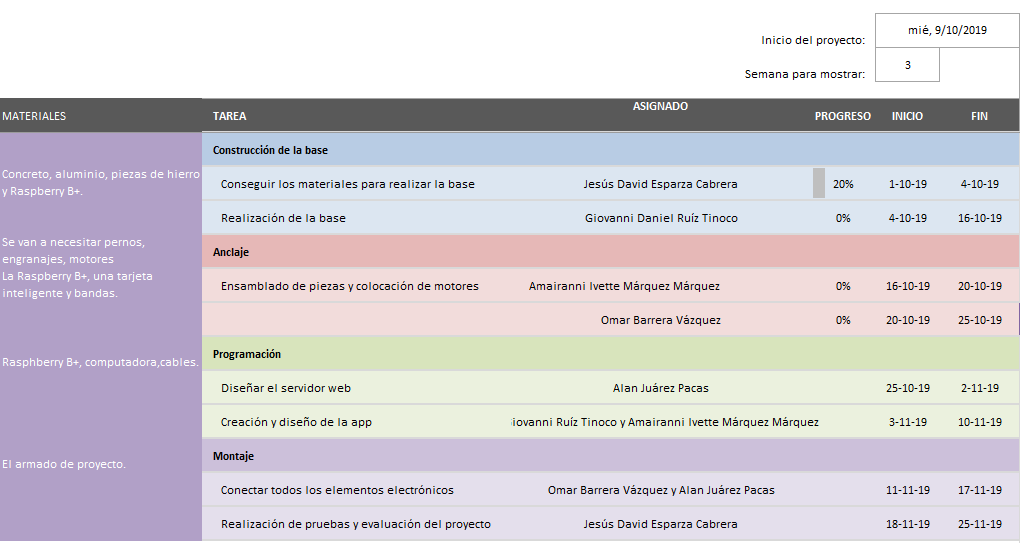
\includegraphics[width=7.11in,height=3.79in]{./media/image2.png}
	\end{Center}
\end{figure}




\par


\vspace{\baselineskip}
\textbf{Calendario }\par




\begin{figure}[H]
	\begin{Center}
		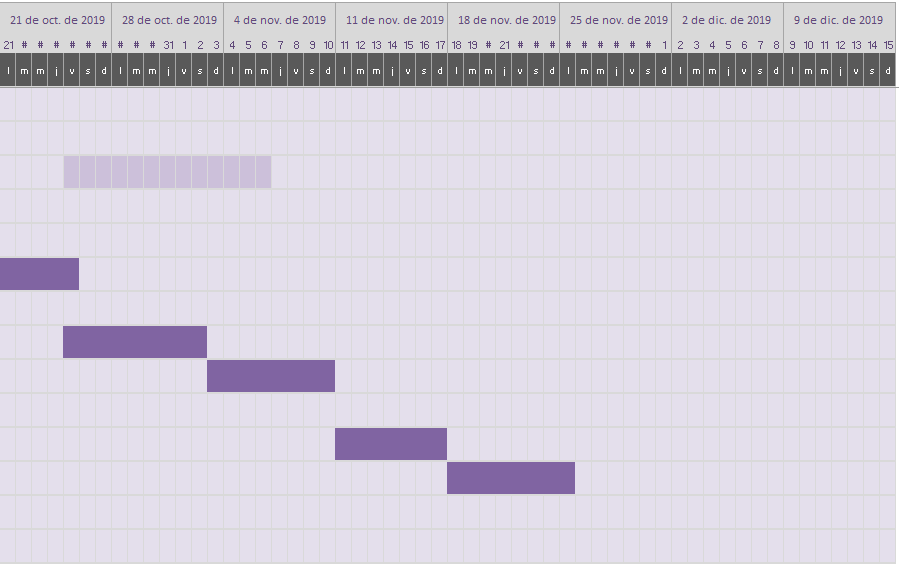
\includegraphics[width=7.18in,height=4.52in]{./media/image3.png}
	\end{Center}
\end{figure}




\par


\vspace{\baselineskip}

\vspace{\baselineskip}

\vspace{\baselineskip}

\vspace{\baselineskip}

\vspace{\baselineskip}

\vspace{\baselineskip}

\vspace{\baselineskip}

\vspace{\baselineskip}

\vspace{\baselineskip}

\vspace{\baselineskip}

\vspace{\baselineskip}

\vspace{\baselineskip}

\vspace{\baselineskip}

\vspace{\baselineskip}

\vspace{\baselineskip}
\newpage
\textbf{Aportación del proyecto en cada una de la asignatura}\par






\begin{table}[H]
 			\centering
\begin{tabular}{p{1.26in}p{4.83in}}
\hline
%row no:1
\multicolumn{1}{|p{1.26in}}{\Centering {\fontsize{10pt}{12.0pt}\selectfont \textbf{Materias de 4to}}} & 
\multicolumn{1}{|p{4.83in}|}{\Centering {\fontsize{10pt}{12.0pt}\selectfont \textbf{Detalles de la Aportación al proyecto}}} \\
\hhline{--}
%row no:2
\multicolumn{1}{|p{1.26in}}{\Centering {\fontsize{10pt}{12.0pt}\selectfont INGLÉS IV}} & 
\multicolumn{1}{|p{4.83in}|}{{\fontsize{10pt}{12.0pt}\selectfont  }Dado que la búsqueda de Datasheets e investigaciones es indispensable un dominio básico del idioma para así podernos documentarnos en ciertos aspectos como las especificaciones de los fabricantes de algunos materiales.} \\
\hhline{--}
%row no:3
\multicolumn{1}{|p{1.26in}}{\Centering {\fontsize{10pt}{12.0pt}\selectfont ÉTICA PROFESIONAL}} & 
\multicolumn{1}{|p{4.83in}|}{{\fontsize{10pt}{12.0pt}\selectfont  }Dado que la búsqueda de Datasheets e investigaciones es indispensable un dominio básico del idioma para así podernos documentarnos en ciertos aspectos como las especificaciones de los fabricantes de algunos materiales.} \\
\hhline{--}
%row no:4
\multicolumn{1}{|p{1.26in}}{\Centering {\fontsize{10pt}{12.0pt}\selectfont ESTRUCTURA Y PROPIEDADES DE LOS MATERIALES}} & 
\multicolumn{1}{|p{4.83in}|}{Con esta materia podemos tener un criterio más amplio sobre las propiedades necesarias en los materiales que son más convenientes para el uso en nuestro proyecto, tomando en cuenta desde resistencia hasta los costos.} \\
\hhline{--}
%row no:5
\multicolumn{1}{|p{1.26in}}{\Centering {\fontsize{10pt}{12.0pt}\selectfont PROGRAMACIÓN DE PERIFÉRICOS}} & 
\multicolumn{1}{|p{4.83in}|}{En esta aprendemos a configurar los sistemas que vamos a usar y a interconectarlos a través del software que nosotros vamos a desarrollar para ser aplicado en este proyecto. \par } \\
\hhline{--}
%row no:6
\multicolumn{1}{|p{1.26in}}{\Centering {\fontsize{10pt}{12.0pt}\selectfont SISTEMAS ELECTRÓNICOS DE INTERFAZ}} & 
\multicolumn{1}{|p{4.83in}|}{Nos ayuda en la realización del análisis de la automatización necesaria para nuestro proyecto, así como en la definición de procesos y operaciones a automatizar también a efectuar el análisis de la función de entrada como el de las funciones de salida las cuales sea necesario integrar o automatizar en el sistema.} \\
\hhline{--}
%row no:7
\multicolumn{1}{|p{1.26in}}{\Centering {\fontsize{10pt}{12.0pt}\selectfont CONTROLADORES LÓGICOS PROGRAMABLES}} & 
\multicolumn{1}{|p{4.83in}|}{{\fontsize{10pt}{12.0pt}\selectfont  }Con los conocimientos que adquiridos en esta materia podemos aplicar en la fase control para los controladores que usaremos en los motores que moverán el sistema mecánico.} \\
\hhline{--}

\end{tabular}
 \end{table}


\newpage


\vspace{\baselineskip}
\textbf{Desarrollo del proyecto }\par

\textbf{\textit{Sistemas electrónicos de interfaz }}\par

En esta materia se ha desarrollado circuitos para el control de elementos de potencia, comenzando desde la primera práctica donde se desarrolló un sistema de control usando optoacopladores para la entrada, relevadores para la salida y un Arduino como CPU, esto es de utilidad en el proyecto para replicarlo en el control de actuadores usando como CPU la raspberry usada previamente en la materia de $``$Programación de periféricos$"$ . Además, en la practica 3 hemos usado un puente H para poder controlar el sentido del giro de un motor, esto es de utilidad para el uso en sistemas móviles que usen motores para el aseguramiento de la motocicleta.\par





\begin{figure}[H]
\advance\leftskip 1.15in		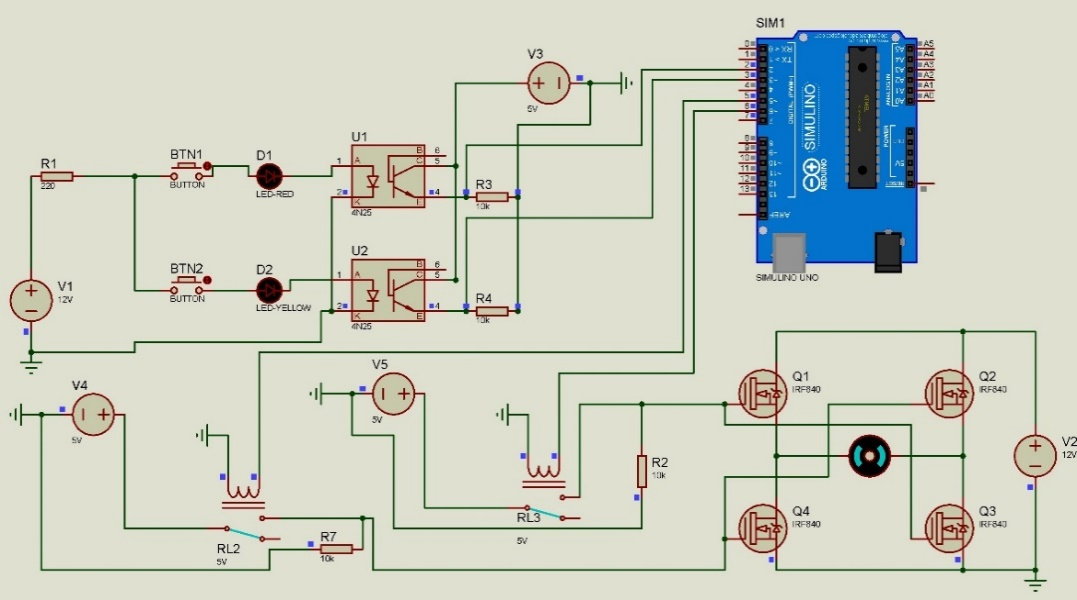
\includegraphics[width=4.91in,height=2.73in]{./media/image4.jpeg}
\end{figure}




\par


\vspace{\baselineskip}

\vspace{\baselineskip}

\vspace{\baselineskip}

\vspace{\baselineskip}

\vspace{\baselineskip}

\vspace{\baselineskip}

\vspace{\baselineskip}

\vspace{\baselineskip}
\newpage
\textbf{Programación de periféricos:}\par








La raspberry pi 3 es un dispositivo que les ayudara a formar un sistema operativo con una combinación de programas con Python. Al utilizar esta combinación nos da la ventaja de tener control del proyecto por medio de comandos y compilación de los pines GPIO que contiene el ordenador de placa reducida. A continuación, se muestra la siguiente figura:

\begin{figure}[H]
\advance\leftskip 0.82in		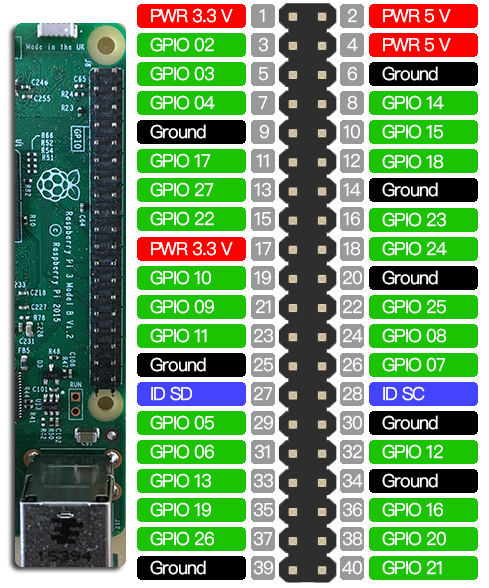
\includegraphics[width=3.06in,height=3.68in]{./media/image5.png}
\end{figure}

\vspace{\baselineskip}
El programa ya mencionado anteriormente $``$Python$"$ , viene instalado por defecto de parte del sistema operativo raspbian, lo utilizara con el fin de controlar el sistema por medio de los pines GPIO estos pines son un sistema de entrada y salida de propósito general, en la materia de programación de perifericos observaron que los pines son de tipo $``$unbuffered$"$ , es decir, no disponen de buffers de protección por lo que puede que dañen el dispositivo con algún mal uso.\par

A base de esta información pueden observar y analizar que pines utilizar durante el proyecto.\par

Al conocer dicha información se puede crear una página web con el uso de Python y otros programas auxiliares que ayuden a darle diseño y estilo a los comandos ordenados por Python.\par


\vspace{\baselineskip}

\vspace{\baselineskip}

\vspace{\baselineskip}

\vspace{\baselineskip}

\vspace{\baselineskip}

\vspace{\baselineskip}

\vspace{\baselineskip}
\newpage
\textbf{Inglés}\par

La mayoría de la información que se ha estado recopilando se encuentra en inglés por tal motivo hacemos uso de nuestros conocimientos adquiridos en esta materia. Así mismo al utilizar la plataforma de GitHub se trabaja con el idioma nativo que es el inglés. \par




\begin{figure}[H]
	\begin{Center}
		
\includegraphics[width=5.23in,height=1.74in]{./media/image6.png}
	\end{Center}
\end{figure}




\par


\vspace{\baselineskip}

\vspace{\baselineskip}
\textbf{Ética profesional}\par

El conocimiento adquirido en esta materia es el trabajar en equipo, respetando las opiniones de todos los integrantes del equipo, del mismo modo enriquecer la información de manera conjunta. \par

En los equipos de trabajo, se elaboran unas reglas, que se deben respetar por todos los miembros del grupo. Son reglas de comportamiento establecidas por los miembros del equipo. Estas reglas proporcionan a cada individuo una base para predecir el comportamiento de los demás y preparar una respuesta apropiada. Incluyen los procedimientos empleados para interactuar con los demás. La función de las normas en un grupo es regular su situación como unidad organizada, así como las funciones de los miembros individuales.\par





\begin{figure}[H]
	\begin{Center}
		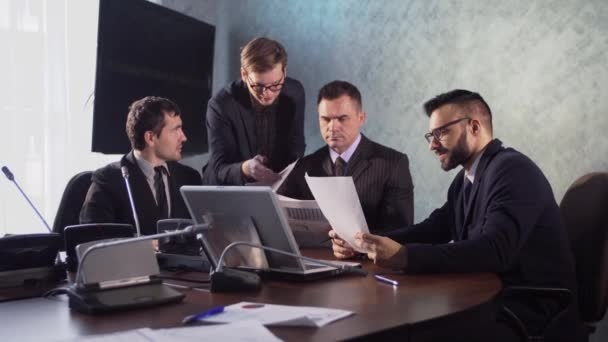
\includegraphics[width=5.3in,height=2.98in]{./media/image7.jpeg}
	\end{Center}
\end{figure}




\par


\vspace{\baselineskip}

\vspace{\baselineskip}

\vspace{\baselineskip}
\textbf{Propiedades y estructuras de los materiales: }\par

Los fines perseguidos por esta asignatura son los siguientes: \par

\begin{itemize}
	\item Permitir al estudiante distinguir el tipo de materiales utilizados en la fabricación de componentes usados en electrónica.\par

	\item Observar las características y aplicaciones específicas de los mismos.\par

	\item Distinguir las nomenclaturas e identificaciones de los componentes.\par

	\item Aplicar las especificaciones y valores nominales indicados por el fabricante. \par

	\item Interpretar acabadamente los parámetros y graficas proporcionadas por el proveedor.\par

	\item Utilizar correctamente la información suministrada para realizar una adecuada selección del componente y su uso correcto. \par

	\item Manejar la información de manera apropiada para realizar una equilibrada selección de componentes de acuerdo a la calidad y el costo de los mismos.
\end{itemize}\par


\vspace{\baselineskip}



\begin{figure}[H]
	\begin{Center}
		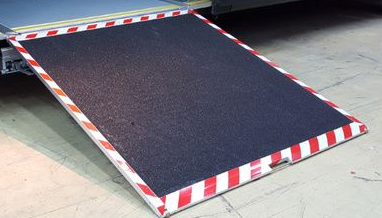
\includegraphics[width=4.53in,height=2.58in]{./media/image8.png}
	\end{Center}
\end{figure}




\par
\newpage
\textbf{Controladores Lógicos Programables}\par


\vspace{\baselineskip}
{\fontsize{11pt}{13.2pt}\selectfont La asignatura de controladores lógicos programables \textit{(PLC) }es utilizada para el proyecto de \textit{$``$Estacionamientos Inteligentes$"$  }el cual nos permitirá el control entre la \uline{interfaz} y \uline{sistemas electrónico de interfaz} por lo cual actuará en la forma de autómata.\par}\par


\vspace{\baselineskip}

\vspace{\baselineskip}
{\fontsize{11pt}{13.2pt}\selectfont La función que llevara el PLC en el proyecto, será poder activar el circuito de potencia que a su vez moverá el mecanismo para controlar el acceso al medio de transporte, la función esta determinara por la siguiente tabla lógica en cuestión del funcionamiento requerido:\par}\par


\vspace{\baselineskip}





\begin{table}[H]
 			\centering
\begin{tabular}{p{1.13in}p{1.02in}p{1.05in}}
%row no:1
\multicolumn{1}{p{1.13in}}{{\fontsize{11pt}{13.2pt}\selectfont A}} & 
\multicolumn{1}{p{1.02in}}{{\fontsize{11pt}{13.2pt}\selectfont B}} & 
\multicolumn{1}{p{1.05in}}{{\fontsize{11pt}{13.2pt}\selectfont C}} \\
\hhline{~~~}
%row no:2
\multicolumn{1}{p{1.13in}}{{\fontsize{11pt}{13.2pt}\selectfont 0}} & 
\multicolumn{1}{p{1.02in}}{{\fontsize{11pt}{13.2pt}\selectfont 0}} & 
\multicolumn{1}{p{1.05in}}{{\fontsize{11pt}{13.2pt}\selectfont 0}} \\
\hhline{~~~}
%row no:3
\multicolumn{1}{p{1.13in}}{{\fontsize{11pt}{13.2pt}\selectfont 0}} & 
\multicolumn{1}{p{1.02in}}{{\fontsize{11pt}{13.2pt}\selectfont 1}} & 
\multicolumn{1}{p{1.05in}}{{\fontsize{11pt}{13.2pt}\selectfont 0}} \\
\hhline{~~~}
%row no:4
\multicolumn{1}{p{1.13in}}{{\fontsize{11pt}{13.2pt}\selectfont 1}} & 
\multicolumn{1}{p{1.02in}}{{\fontsize{11pt}{13.2pt}\selectfont 0}} & 
\multicolumn{1}{p{1.05in}}{{\fontsize{11pt}{13.2pt}\selectfont 0}} \\
\hhline{~~~}
%row no:5
\multicolumn{1}{p{1.13in}}{{\fontsize{11pt}{13.2pt}\selectfont 1}} & 
\multicolumn{1}{p{1.02in}}{{\fontsize{11pt}{13.2pt}\selectfont 1}} & 
\multicolumn{1}{p{1.05in}}{{\fontsize{11pt}{13.2pt}\selectfont 1}} \\
\hhline{~~~}

\end{tabular}
 \end{table}



\vspace{\baselineskip}
{\fontsize{11pt}{13.2pt}\selectfont Esta tabla es la seleccionada para la lógica del autómata dado que la función de entrada que se tienen que activar son la de la ubicación en la que se tiene que posicionar la motocicleta y el sensor que confirma el estado de cerrado.\par}\par


\vspace{\baselineskip}
{\fontsize{11pt}{13.2pt}\selectfont Estas dos aplicaciones son adquiridas de la asignatura de PLC, la cual demuestra la utilización de sensores y actuadores. Además de estas dos entradas serán utilizadas entradas de sensores de movimiento (nivel de presionan a vibraciones menores a mayores) conectadas al autómata en el cual responderá por medio de sus salidas con actuadores, alarmas al sistema de interfaz de usuario programado para estar en la WEB.\par}\par


\vspace{\baselineskip}
{\fontsize{11pt}{13.2pt}\selectfont Representación del circuito de simulador $``$Proteus$"$  figura 1.:\par}\par


\vspace{\baselineskip}


%%%%%%%%%%%%%%%%%%%% Figure/Image No: 9 starts here %%%%%%%%%%%%%%%%%%%%

\begin{figure}[H]
	\begin{Center}
		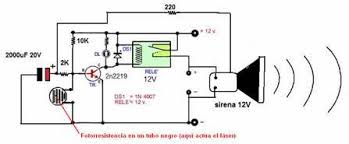
\includegraphics[width=5.06in,height=1.88in]{./media/image9.png}
	\end{Center}
\end{figure}


%%%%%%%%%%%%%%%%%%%% Figure/Image No: 9 Ends here %%%%%%%%%%%%%%%%%%%%

\par


\vspace{\baselineskip}

\vspace{\baselineskip}

\vspace{\baselineskip}

\vspace{\baselineskip}

\vspace{\baselineskip}

\vspace{\baselineskip}

\vspace{\baselineskip}

\vspace{\baselineskip}

\vspace{\baselineskip}

\vspace{\baselineskip}
{\fontsize{11pt}{13.2pt}\selectfont La parte de entradas y salidas de alimentación estarán conectadas al autómata, por lo que nos serviré como un actuado en caso de intento de robo, el sistema de notificaciones es algo en lo que aun se trabaja al no tener definido el proceso con el cual se tomaran o descartaran algunas alarmas.\par}\par


\vspace{\baselineskip}
{\fontsize{11pt}{13.2pt}\selectfont \textbf{Cierre y apertura del perno de sujeción con PLC.}\par}\par


\vspace{\baselineskip}
{\fontsize{11pt}{13.2pt}\selectfont El cierre y apertura estará determinado por el proceso de control del PLC el cual determinara si esta permanece cerrado o abierto y por cuanto tiempo, por lo que eso lo indicara el procesador del autómata, el cual será sujeto a las condiciones que se le otorguen en cuanto a los tiempos, algo parecido al circuito elaborado con la asignatura de \textbf{controladores lógicos programables }en la cual se hace la función de un autómata y el encendido lógico, como lo muestra la figura 2\par}\par


\vspace{\baselineskip}


%%%%%%%%%%%%%%%%%%%% Figure/Image No: 10 starts here %%%%%%%%%%%%%%%%%%%%

\begin{figure}[H]
\advance\leftskip 0.27in		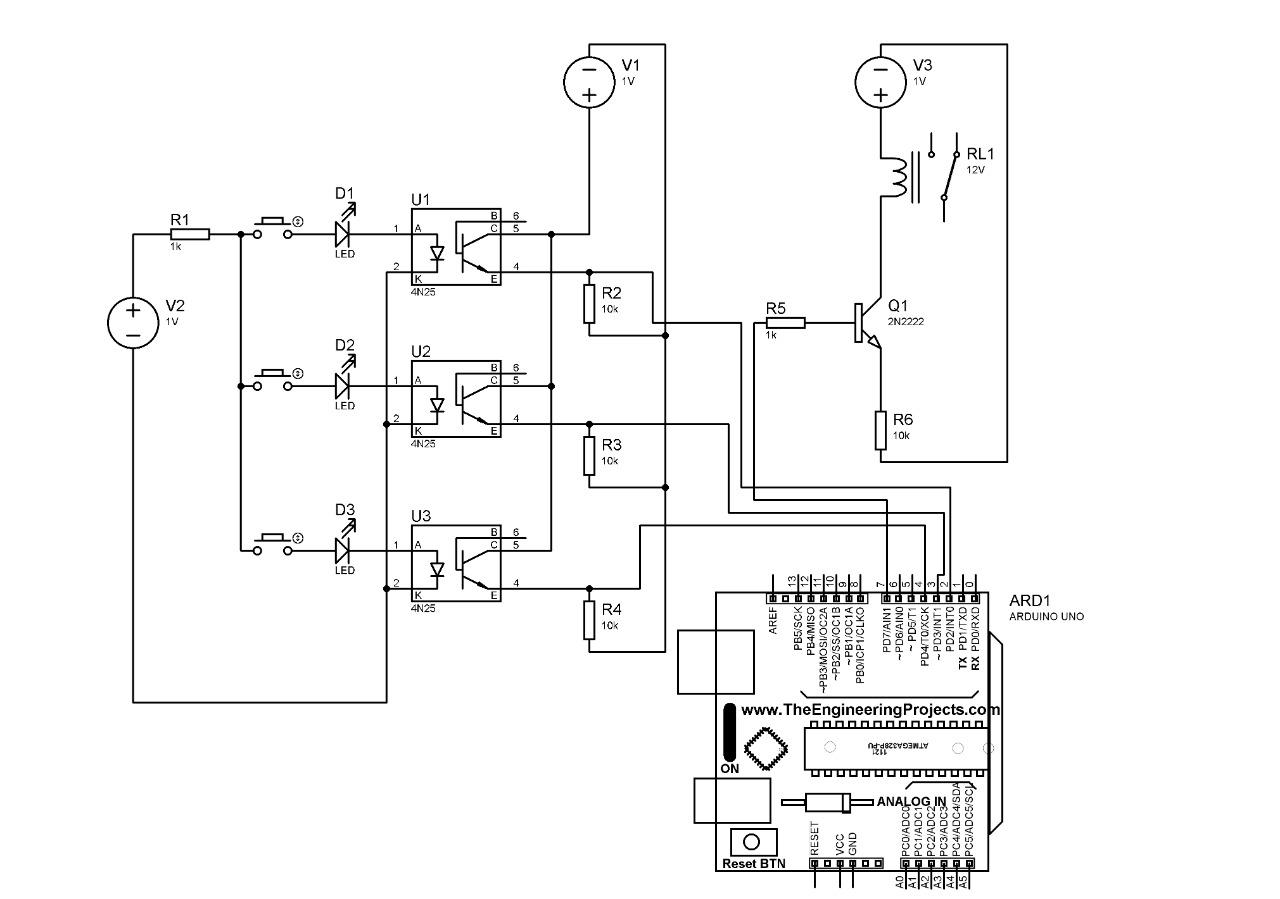
\includegraphics[width=6.91in,height=3.06in]{./media/image10.png}
\end{figure}


%%%%%%%%%%%%%%%%%%%% Figure/Image No: 10 Ends here %%%%%%%%%%%%%%%%%%%%

\par


\vspace{\baselineskip}

\vspace{\baselineskip}
\textbf{Bibliografía }\par

\textit{El informador. (2019). En tres años se duplica robo de motos con violencia en Jalisco. 09/10/19, de El Informador Sitio web: En tres años se duplica robo de motos con violencia en Jalisco}\par

Notimex. (2019).Estas son las motocicletas más robadas del país 09/10/19, de El universal Sitio web: \href{https://www.eluniversal.com.mx/cartera/economia/estas-son-las-motocicletas-mas-robadas-en-el-pais}{https://www.eluniversal.com.mx/cartera/economia/estas-son-las-motocicletas-mas-robadas-en-el-pais}\par

Jorge Martínez. (2018). Roban 6 motocicletas al día en Jalisco: FGE. 09/10/19, de Milenio Sitio web: \href{https://www.milenio.com/politica/comunidad/roban-6-motocicletas-al-dia-en-jalisco-fge}{https://www.milenio.com/politica/comunidad/roban-6-motocicletas-al-dia-en-jalisco-fge}\par


\printbibliography
\end{document}